\chapter{Улучшения бинарного оптимизатора BOLT}\label{ch:ch3}
Данная глава посвящена вопросам улучшения бинарного оптимизатора BOLT под ARM архитектуру.

В разделе 3.1 рассматривается проблема длинных переходов в бинарной оптимизации. Предлагается метод оптимизации трамплинов, позволяющий уменьшить количество добавляемых для трамплина инструкций и не использовать дополнительный регистр.

В разделе 3.2 обсуждается проблема бинарной оптимизации исполняемых файлов под ARM архитектуру, в которых используются таблицы переходов. Предлагается метод обхода данной проблемы.

В разделе 3.3 предлагается метод верификации оптимизированного бинарного файла. Приводится описание разработанного формата преобразования, позволяющего проверить корректность перекомпоновки кода. Приводятся разработанные правила верификации и разрешенные преобразования. Показаны результаты верификации и найденные ошибки.

В разделе 3.4 описываются результаты тестирования синтетических тестов и общих наборов тестов после оптимизации модифицированным бинарным транслятором BOLT.

\section{Оптимизация длинных переходов}\label{sec:ch3/sect1}
Помимо отсутствия LBR, ARM архитектура накладывает дополнительные ограничения на перемещение горячих базовых блоков. Перекомпоновка кода проще реализуется на CISC архитектуре за счёт возможности добавления длинных прыжков одной инструкцией. На RISC архитектурах количество битов смещения в инструкциях переходов меньше, что приводит к ограничению диапазона возможного перемещения. Также инструкция загрузки в регистр адреса, который зависит от счетчика инструкций, на ARM архитектуре ограничена 20 битами, выделенными на смещение, и накладывает возможный диапазон перемещения ± 1 мегабайт (рисунок \cref{fig:CmpPcRel}). Все инструкции, зависящие от адреса инструкции (переходы, загрузка адреса, загрузка по регистру/смещению) после оптимизации необходимо проверить на возможность записи нового смещения в отведенные для этого биты \cite{Blem2013} \cite{confbib1}.

\begin{figure}[ht]
    \centerfloat{
        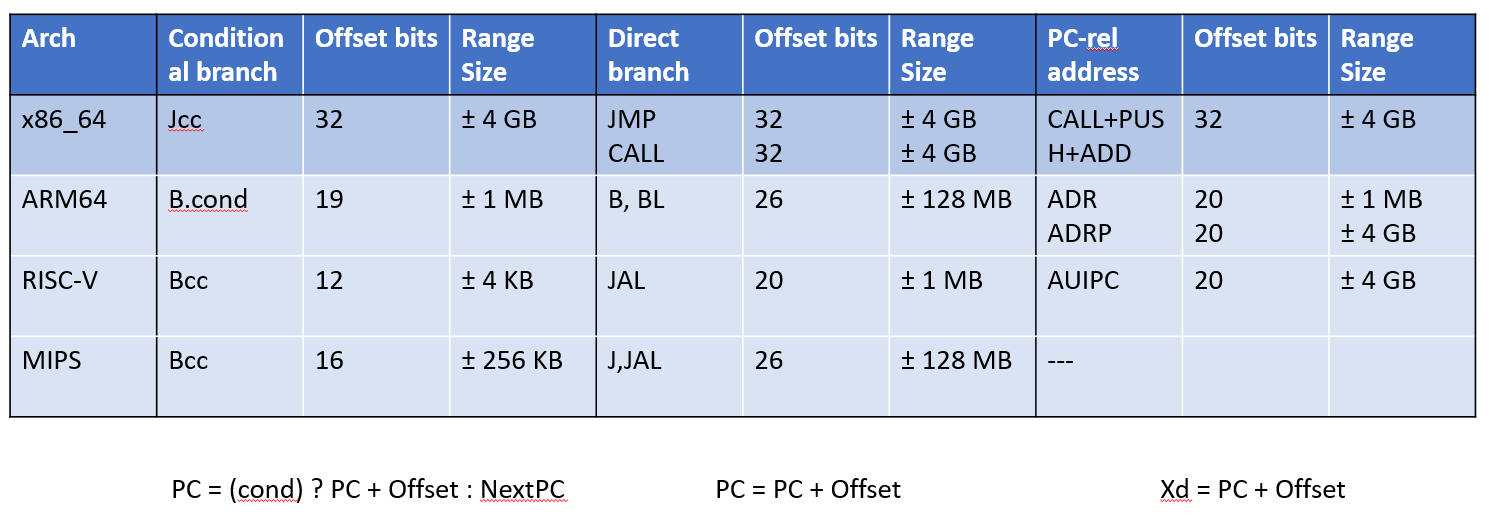
\includegraphics[width=1.0\linewidth]{pcrel}
    }
    \caption{Сравнение инструкций, зависящих от счетчика инструкций}\label{fig:CmpPcRel}
\end{figure}

Таким образом, при перемещении горячего кода, который ссылается на холодный участок (черная стрелка), происходит переполнение значения смещения и оптимизация становится некорректной (рисунок \cref{fig:HotMove}).

\begin{figure}[ht]
    \centerfloat{
        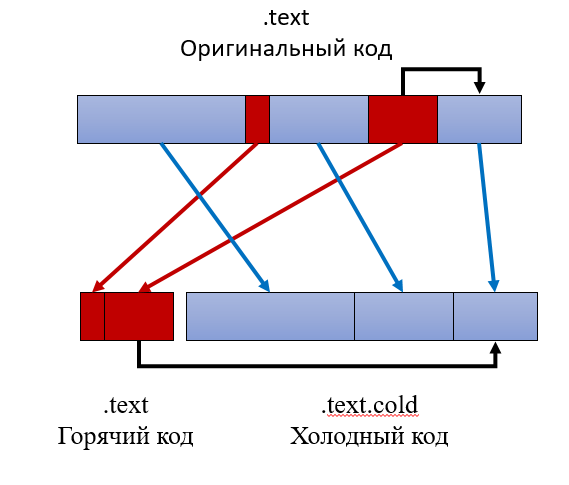
\includegraphics[width=0.8\linewidth]{11}
    }
    \caption{Пример перекомпоновки горячего кода}\label{fig:HotMove}
\end{figure}

Для решения данной проблемы необходимо добавить трамплин – дополнительный код, позволяющий генерировать произвольный адрес и произвести переход либо загрузку по данному значению (рисунок \cref{fig:Tramp}). Подобное решение будет увеличивать размер кода, что приведёт к понижению производительности, при этом диапазон перемещаемого кода будет увеличен. Также необходимо наличие свободного регистра, в который будет записываться данный адрес.

\begin{figure}[ht]
    \centerfloat{
        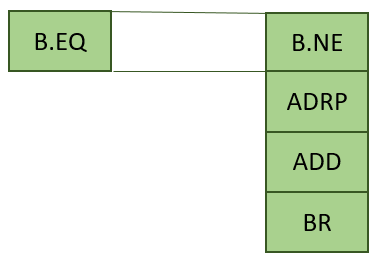
\includegraphics[width=0.5\linewidth]{opt3}
    }
    \caption{Генерация трамплина для инструкции условного перехода}\label{fig:Tramp}
\end{figure}

Альтернативный подход – генерация таблицы трамплинов рядом с горячим кодом. Таким образом, поток управления будет проходить через неё в случае прыжка из горячего кода в холодный. Данный подход решит проблему инструкций переходов без увеличения размера горячего кода. В обратном направлении можно вставлять трамплины прямо в холодный код, так как его размер не сильно повлияет на изменение производительности.

Для условных переходов можно написать маленькие трамплины размером в одну инструкцию с помощью добавления одного безусловного перехода, если смещение занимает больше 19, но меньше 26 бит (рисунок \cref{fig:CmpBranch}).

\begin{figure}[ht]
    \centerfloat{
        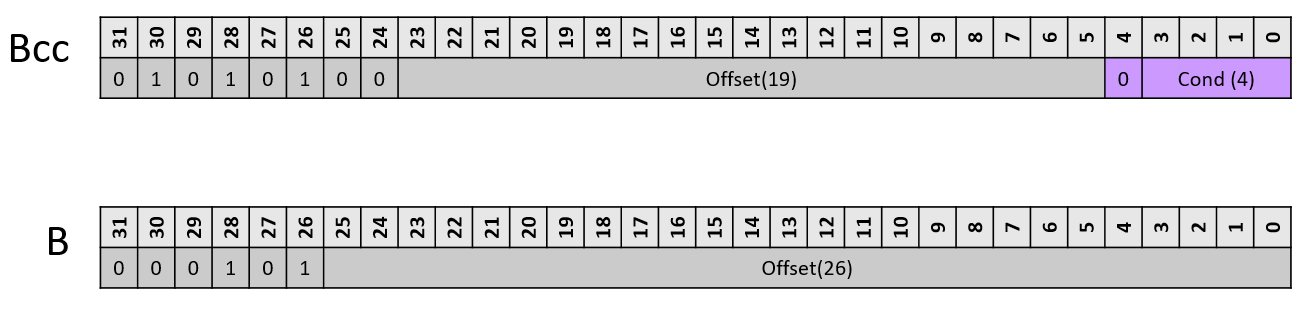
\includegraphics[width=1.0\linewidth]{opt1}
    }
    \caption{Сравнение условного и безусловного перехода}\label{fig:CmpBranch}
\end{figure}

\begin{figure}[ht]
    \centerfloat{
        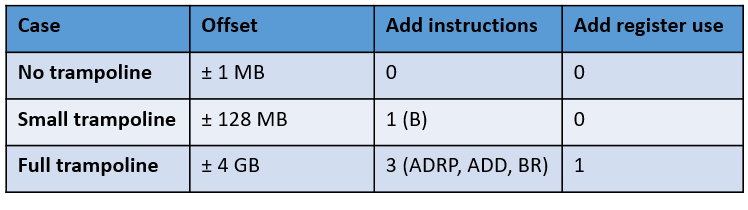
\includegraphics[width=1.0\linewidth]{opt4}
    }
    \caption{Сравнение трамплинов}\label{fig:CmpTramp}
\end{figure}

В этом случае необходимо инвертировать условие инструкции, а метку для прыжка поставить через одну инструкцию прямого перехода, вставленную оптимизатором непосредственно после условного перехода (рисунок \cref{fig:CmpTramp}). В результате региона перемещения увеличивается в 128 раз за счёт отличий в кодировке Bcc и B, а увеличение кода произошло всего на 1 инструкцию (рисунок \cref{fig:ExTramp}).
 
\begin{figure}[ht]
    \centerfloat{
        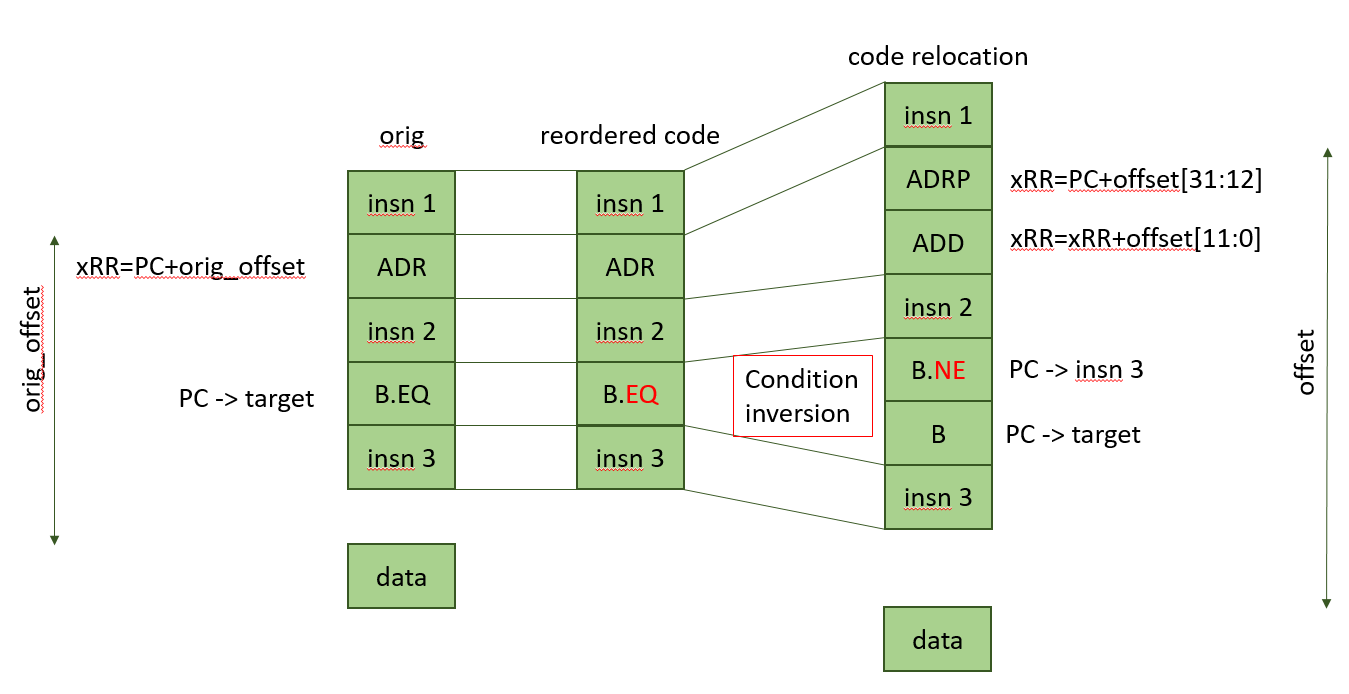
\includegraphics[width=1.0\linewidth]{opt2}
    }
    \caption{Схема добавления трамплинов для ADR (сверху) и Bcc (снизу) инструкций}\label{fig:ExTramp}
\end{figure}

В верхней части рисунка \cref{fig:ExTramp} изображено решение для ADR инструкции. Если увеличение смещения больше возможного, инструкция заменяется на пару ADRP+ADD, это увеличивает возможный регион перемещений с 1 мегабайт до 4 гигабайт и покрывает все необходимые расстояния.
И последний тип инструкций, зависящий от адреса команды - загрузки по регистру/смещению. В простейшем варианте проблемы с большим смещением решается добавлением одной инструкции ADR.
Данные подходы позволили оптимизировать большинство приложений, при добавлении лишь одной дополнительной инструкции на каждый случай.

\section{Исправление преобразования таблиц переходов}\label{sec:ch3/sect2}

Помимо проблем с недостаточным количеством битов в инструкциях на ARM архитектуре, была найдена проблема с таблицей переходов (jump table). При перемещении кода конкретного варианта конструкции switch-case необходимо модифицировать запись в таблице, используемую в косвенном переходе. Оптимизатор узнает адрес записи из релокационной информации, которая для некоторых случаев кода ARM архитектуры не будет корректной. Это происходит по причине несоответствия адреса, от которого вычисляется целевой адрес для прыжка при исполнении и генерации релокационной информации.

Рассмотрим пример, приведенный на рисунке \cref{fig:SC1}. Конструкция switch-case реализуется через трамплин на код конкретного case-кода, расположенного по адресу \textbf{CASE2\_ADR}. За 3 инструкции (ADD, LDR, ADD) происходит вычисление этого адреса в регистре X2, а четвертой инструкцией BR - перемещение на код case2.

Для вычисления этого адреса предварительно были подготовлены следующие значения: регистр X0 - номер рассматриваемого case, регистр X1 - адрес начала таблицы переходов, память по адресу \textbf{JTR2\_ADR} - смещение относительно данного адреса до \textbf{<case2 code>} \textbf{JTR2\_VAL}.

Вычисление регистра X2 для перехода по нему происходит в три этапа:
\begin{enumerate}[beginpenalty=10000]
  \item Вычисление \textbf{JTR2\_ADR} в регистре X3.
  \item Загрузка значения \textbf{JTR2\_VAL} в регистр X2.
  \item Вычисление \textbf{CASE2\_ADR} в регистре X2.
\end{enumerate}


\begin{figure}[!h]
    \centerfloat{
        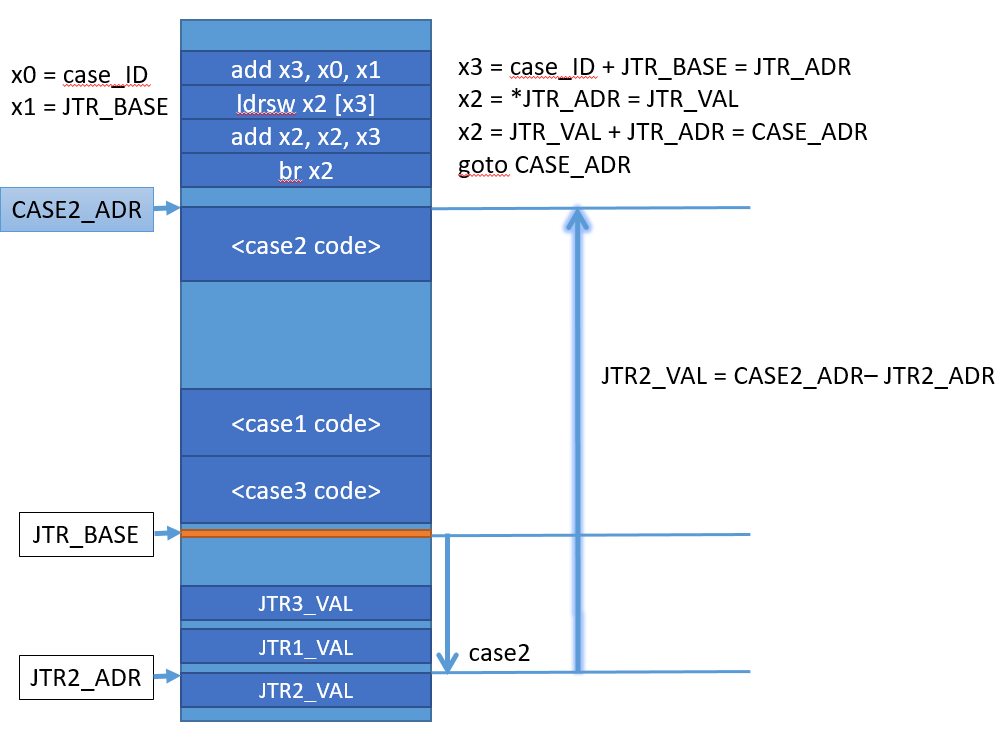
\includegraphics[width=1.0\linewidth]{jt2}
    }
    \caption{Пример ассемблерного кода для switch-case случая}\label{fig:SC1}
\end{figure}

В бинарном файле есть специальная релокационная секция, где записана вся информация об инструкциях и данных, зависящих от счетчика инструкций (PC-relative). В данном примере таким значением является  \textbf{JTR2\_VAL}. Для него записываются три поля релокационной записи: адрес, тип (PREL32 -- PC Relative 32 bit) и в нём хранящееся значение. Для \textbf{JTR2\_VAL} запись приведена на рисунке \cref{fig:Rel1}.

\begin{figure}[!h]
    \centerfloat{
        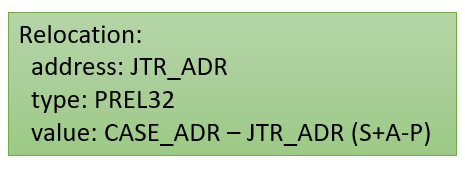
\includegraphics[width=0.6\linewidth]{jt_1}
    }
    \caption{Заполненная структура релокационной записи для перехода по значению регистра}\label{fig:Rel1}
\end{figure}

Релокационная информация необходима для того, чтобы после перестановки кода в бинарном файле можно было переписать все значения, зависящие от счетчика инструкций. На рисунке \cref{fig:SC2} приведен пример перемещения \textbf{<case2 code>}, в результате которого \textbf{JTR2\_VAL} будет переписан, чтобы указывать на новое местоположение кода (зеленые поля).

\begin{figure}[!h]
    \centerfloat{
        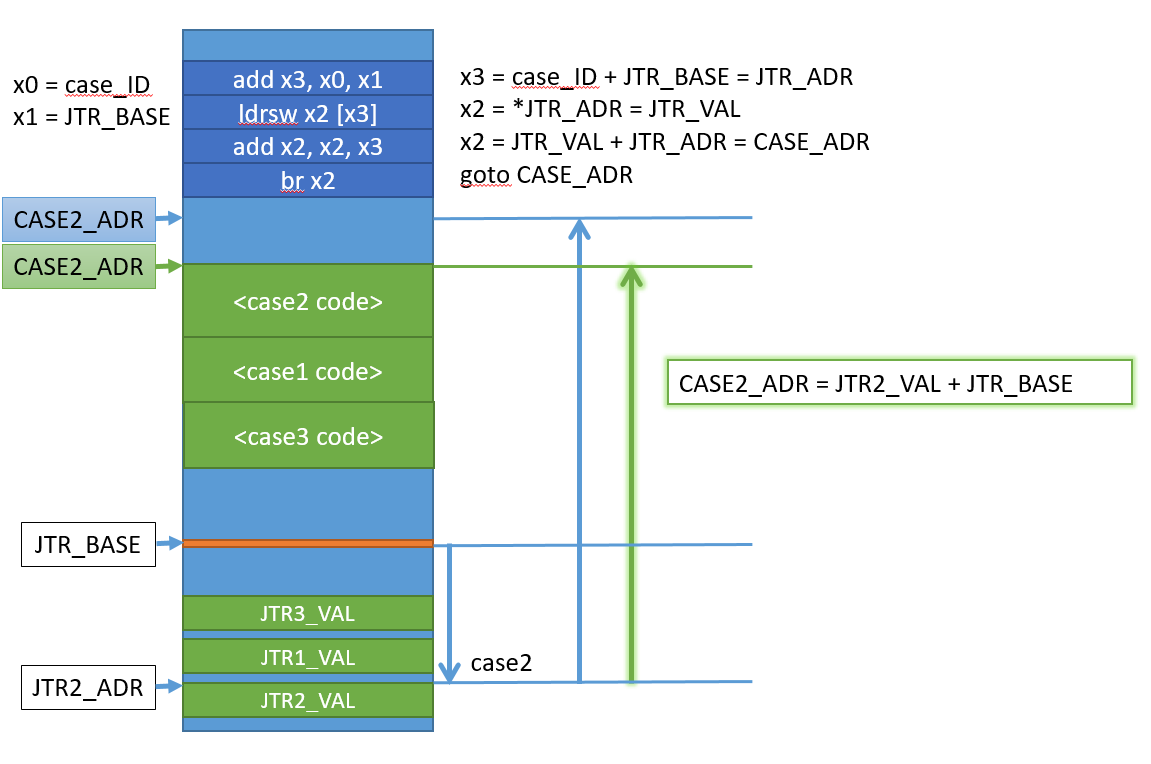
\includegraphics[width=1.0\linewidth]{jt3}
    }
    \caption{Преобразование смещений при перекомпоновке кода}\label{fig:SC2}
\end{figure}

На ARM архитектуре возможно произвести оптимизацию данного примера, уменьшив на одну инструкцию процесс вычисления адреса \textbf{CASE2\_ADR} и освободив один регистр (рисунок \cref{fig:SC3}). Для этого необходимо хранить в таблице переходов смещения не между кодом case и записью в таблице переходов, а между кодом case и началом таблицы перехода. В этом случае второй этап подготовки адреса \textbf{CASE2\_ADR} будет использовать инструкцию LDR, которая будет загружать данные по результату сложения регистров X0 и X1. Тогда первое сложение тогда будет не нужно, и освободится регистр X3, в который до этого записывалось значение \textbf{JTR2\_ADR}.

\begin{figure}[!h]
    \centerfloat{
        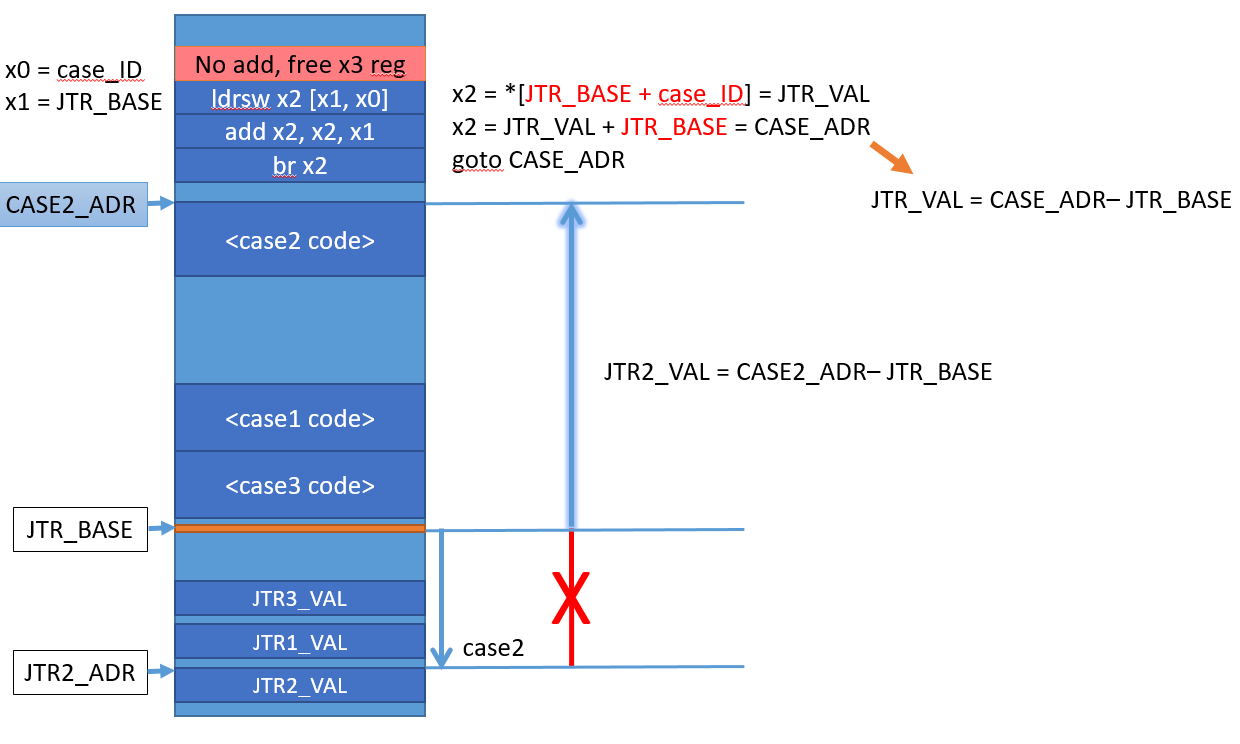
\includegraphics[width=1.0\linewidth]{jt4}
    }
    \caption{Оптимизированный вариант ассемблерного кода для switch-case случая}\label{fig:SC3}
\end{figure}

При данной оптимизации запись в релокационной секции станет не корректной, так как теперь записанный адрес \textbf{JTR2\_ADR} не соответствует базе, от которой отсчитывается  смещение до \textbf{<case2 code>} (рисунок \cref{fig:Rel2}).

\begin{figure}[!h]
    \centerfloat{
        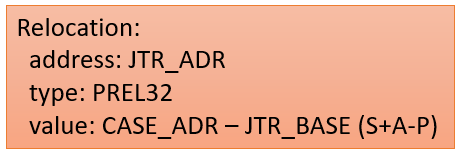
\includegraphics[width=0.6\linewidth]{jt_2}
    }
    \caption{Оптимизированный вариант структуры релокационной записи для перехода по значению регистра}\label{fig:Rel2}
\end{figure}

В данном случае бинарный оптимизатор, прочитав релокационную секцию, будет воспринимать смещение не относительно начала таблицы переходов, а относительно записи в таблице (рисунок \cref{fig:SC4}), и произойдёт смещение на значение \textbf{case\_ID}. То есть релокационная запись указывает на какой-то случайный код \textbf{<some code>} по адресу \textbf{CASE2\_REL}.

\begin{figure}[!h]
    \centerfloat{
        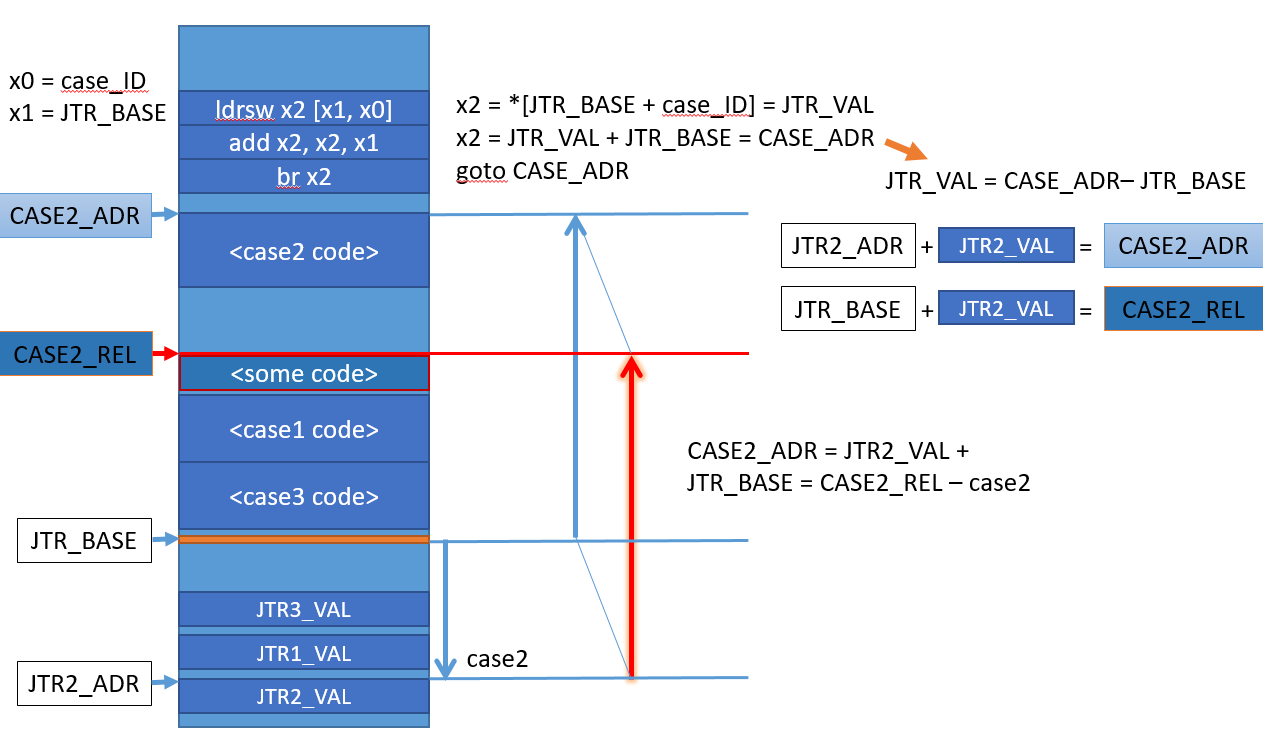
\includegraphics[width=0.8\linewidth]{jt5}
    }
    \caption{Ошибочный расчет целевого адреса бинарным оптимизатором}\label{fig:SC4}
\end{figure}

Когда будет происходить перекомпоновка кода, бинарным оптимизатором будет отслеживаться неверный код, из-за чего таблица переходов будет модифицирована некорректно, если \textbf{<some code>} сместится относительно \textbf{<case2 code>} (рисунок \cref{fig:SC5}).

\begin{figure}[!h]
    \centerfloat{
        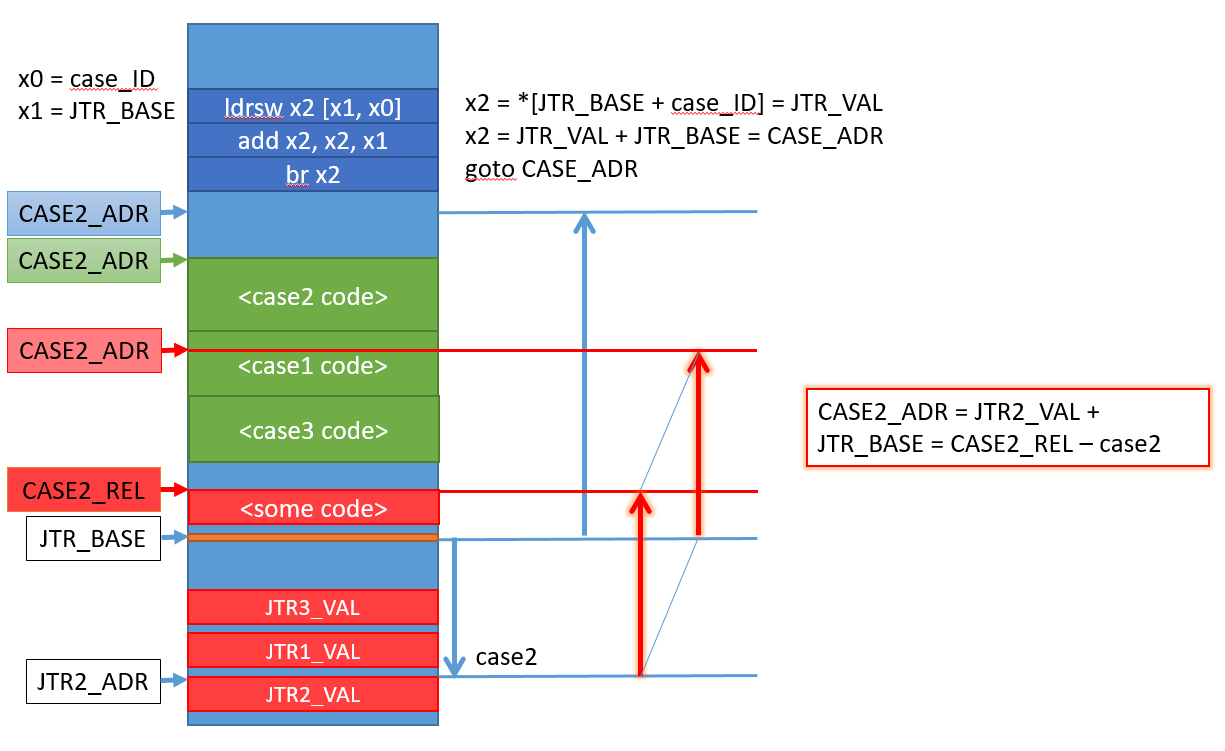
\includegraphics[width=1.0\linewidth]{jt6}
    }
    \caption{Преобразование смещений при перекомпоновке оптимизированного кода}\label{fig:SC5}
\end{figure}

Данная проблема была найдена при оптимизации бинарного файла набора тестов GeekBench (рисунок \cref{fig:SCEx1}). Оптимизация обработки switch-case случая компилятором привела к некорректной релокационной записи и ошибочной модификации записи таблицы перехода (рисунок \cref{fig:SCEx2}).

\begin{figure}[!h]
    \centerfloat{
        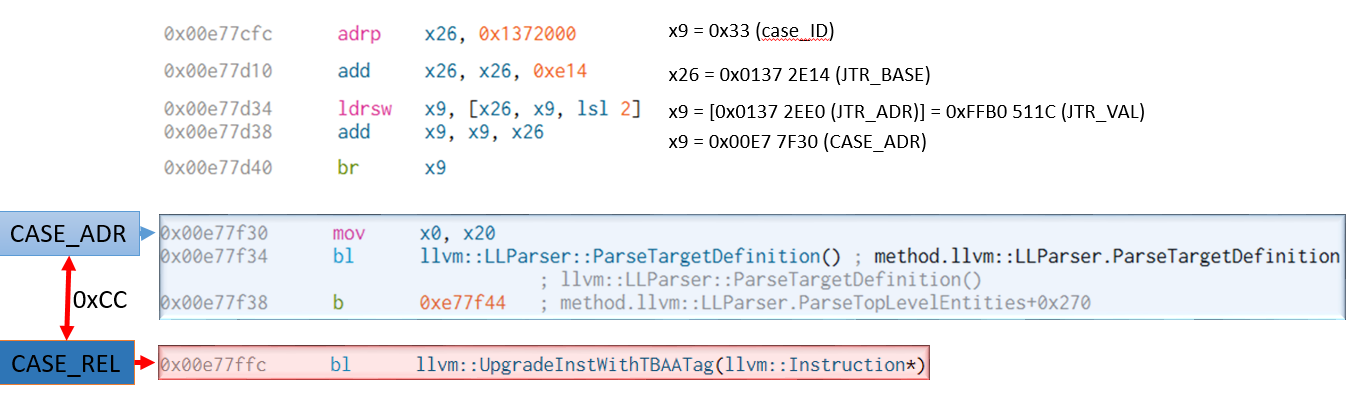
\includegraphics[width=1.0\linewidth]{jt7}
    }
    \caption{Пример кода с переходом по значению регистра (тестовый набор GeekBench)}\label{fig:SCEx1}
\end{figure}

\begin{figure}[!h]
    \centerfloat{
        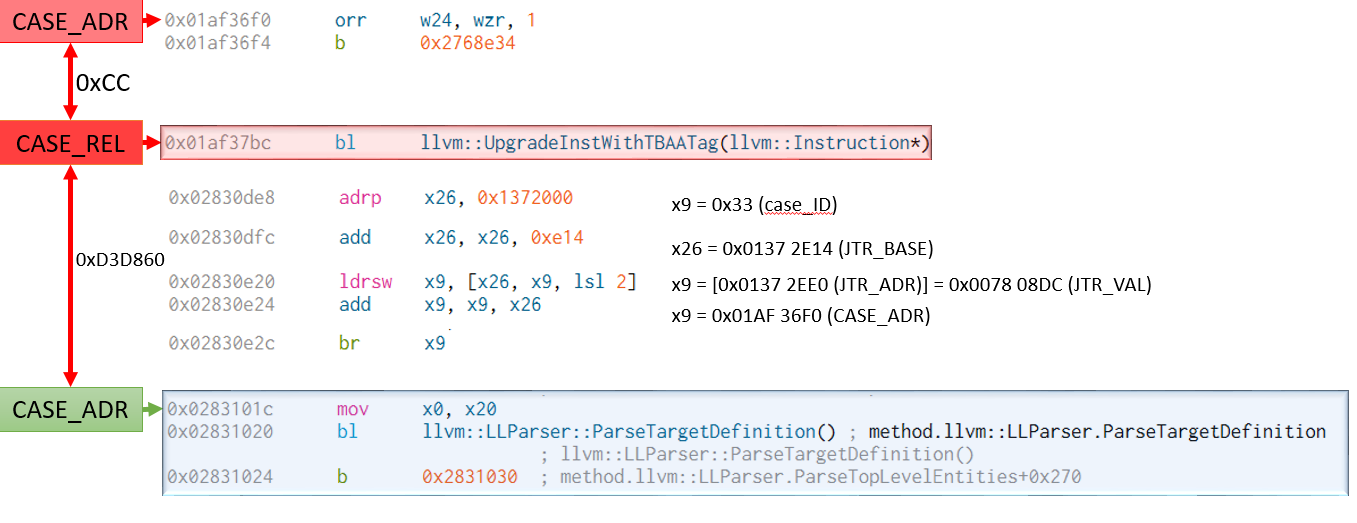
\includegraphics[width=1.0\linewidth]{jt8}
    }
    \caption{Пример кода с переходом по значению регистра после перекомпоновки(тестовый набор GeekBench)}\label{fig:SCEx2}
\end{figure}

Данная проблема была решена переиспользованием оригинального участка кода с данным косвенным переходом. То есть необходимо сохранить копию оригинальной секции .bolt.org.text, так как вычислить из данных релокационной записи адрес начала таблицы переходов в общем случае невозможно.

\section{Верификация бинарной оптимизации}\label{sec:ch3/sect3}
В результате работы бинарного оптимизатора BOLT генерируется новый исполняемый файл, в котором добавлены новые оптимизированные секции. Этот файл показывает лучшие характеристики производительности в сравнении с оригинальным, но помимо перестановки кода есть возможность провести другие оптимизации как общие, так и микроархитектурные. BOLT позволяет дописывать дополнительные проходы, соответствующие новым оптимизациям, но усложнение транслятора ведёт к более сложной отладке возможных проблем и верификации полученного оптимизированного исполняемого файла.

Для решения данной задачи было предложено разработать специальный формат, описывающий преобразования исполняемого файла в оптимизированный, так называемый remap-файл (рисунок \cref{fig:Remap}). В нём записывается информация о всех совершенных перестановках кода и дополнительная информация, обозначающая инструкции, подвергнутые преобразованиям в процессе перекомпоновки (PC-relative инструкции).


\begin{figure}[!h]
    \centerfloat{
        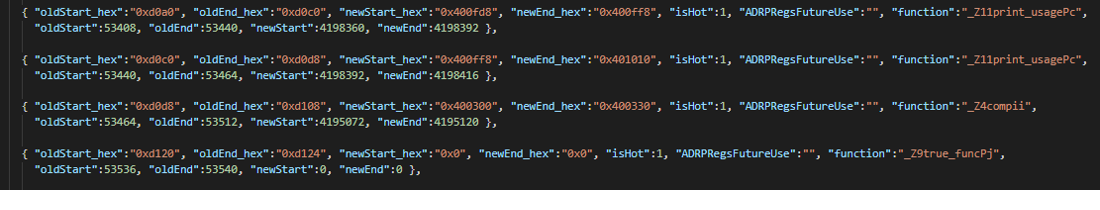
\includegraphics[width=1.0\linewidth]{v1}
    }
    \caption{Пример файла преобразований бинарного файла}\label{fig:Remap}
\end{figure}

Каждая запись относится к одному линейному участку и включает в себя новые и старые начальные и конечные адреса в бинарном файле. Соответствующие начальный и конечный адреса могут совпадать, указывая на пустой блок. Это возможно, если оптимизатор удаляет линейный участок или добавляет новый. Атрибуты с суффиксом <<\_hex>> - это строки с шестнадцатеричным представлением значений в соответствующих атрибутах без суффикса, которые применяются для отладки. <<isHot>> равен 1, если линейный участок часто используемый и был перемещен в секцию горячего кода.

\begin{figure}[!h]
    \centerfloat{
        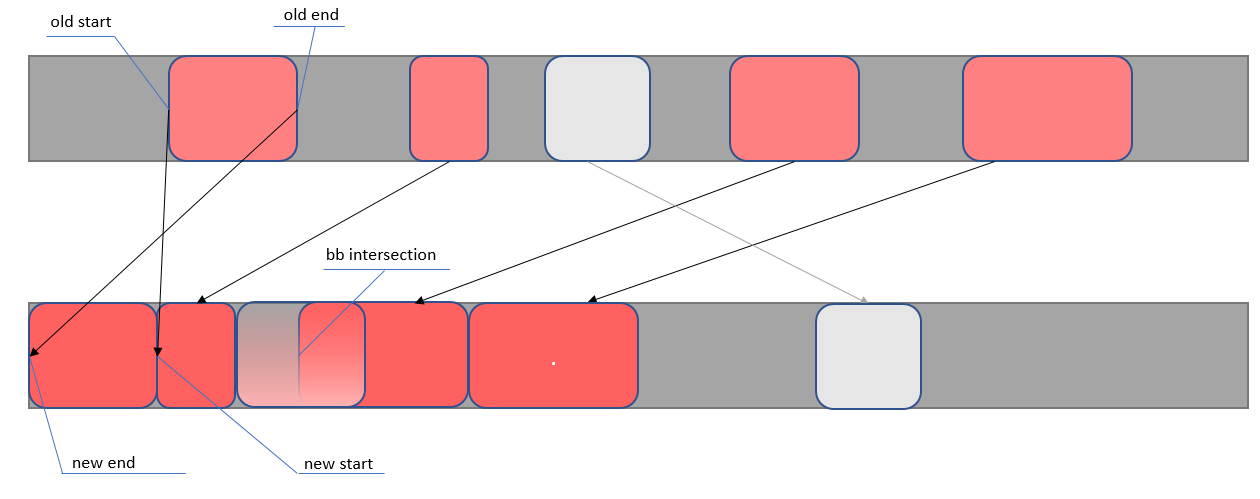
\includegraphics[width=1.0\linewidth]{v2}
    }
    \caption{Схема верификации бинарного файла}\label{fig:Verif}
\end{figure}

В рамках данной работы в BOLT был добавлен проход, генерирующий remap-файл, а также написан статический анализатор, сравнивающий оригинальный и оптимизированный исполняемые файлы по данному remap-файлу (рисунок \cref{{fig:Verif}}). Реализованы следующие проверки:

\begin{enumerate}[beginpenalty=10000]
  \item Проверка корректности оптимизированных линейных участков кода.
  \item Проверка корректности создания теневых точек.
  \item Сравнение инструкций оптимизированных и исходный линейных участков.
\end{enumerate}	

\begin{figure}[!h]
    \centerfloat{
        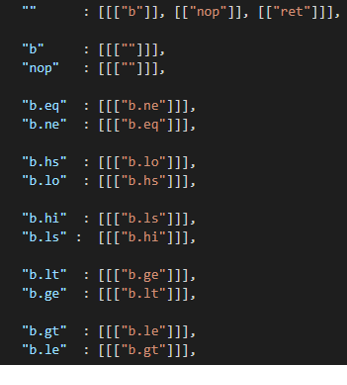
\includegraphics[width=0.6\linewidth]{v3}
    }
    \caption{Пример файла разрешенных преобразований}\label{fig:Access}
\end{figure}

Последний тип проверки использует файл разрешенных преобразований, где описывается преобразования линейного участка (рисунок \cref{fig:Access}).

\begin{figure}[!h]
    \centerfloat{
        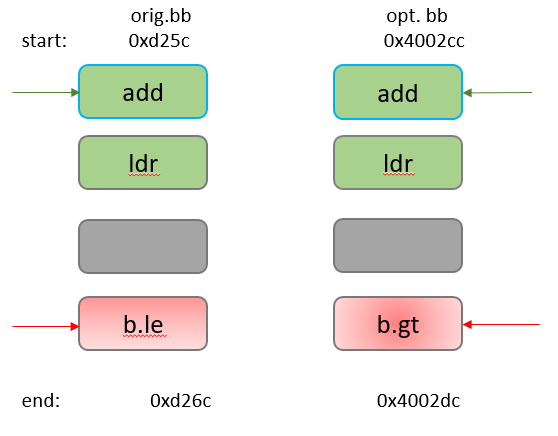
\includegraphics[width=0.6\linewidth]{v4}
    }
    \caption{Проверка линейного участка без изменения количества инструкций}\label{fig:VerifEx1}
\end{figure}

Проверка запускает рекурсивный анализ преобразования линейного участка, последовательно набирая разрешенные преобразования до тех пор, пока линейные участки не совпадут (рисунки \cref{fig:VerifEx1} и  \cref{fig:VerifEx2}).

\begin{figure}[!h]
    \centerfloat{
        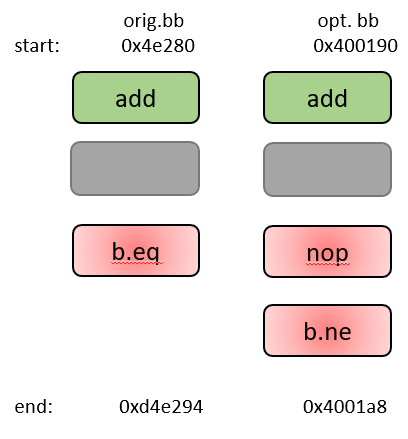
\includegraphics[width=0.5\linewidth]{v5}
    }
    \caption{Проверка линейного участка с измененным количества инструкций}\label{fig:VerifEx2}
\end{figure}

В результате проделанной работы была обеспечена статическая верификация оптимизированных BOLT-ом приложений, что обеспечило выявление ошибок оптимизатора на наборах тестов SPEC CPU 2017 и GeekBench.

\section{Результаты тестирования модифицированного оптимизатора}\label{sec:ch3/sect4}
Реализованный метод генерации профиля и модифицированная версия BOLT для ARM архитектуры были протестированы на описанных выше синтетических тестах.

Для проверки оптимизации на реальном приложении был выбран набор тестов производительности GeekBench. Среди всего набора был выбран тест с наибольшим числом iTLB и L1I промахов – Clang. При компиляции набора тестов были использован флаг <<-O2>>, который соответствует оптимизациям при стандартной сборке приложений \cite{vakbib1}.

\begin{figure}[!h]
    \centerfloat{
        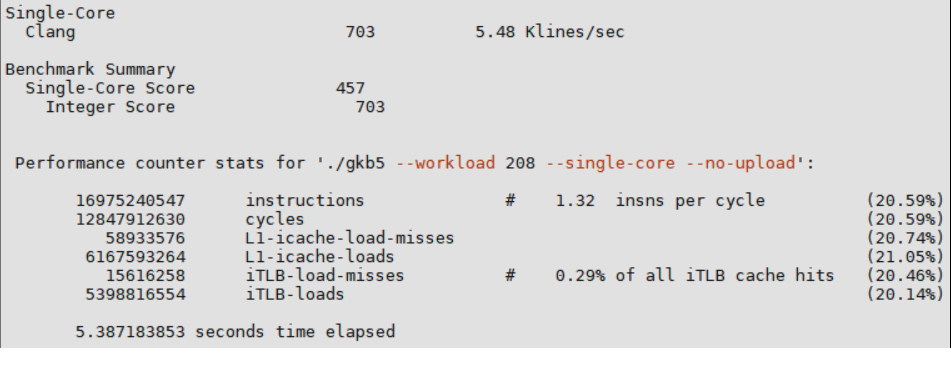
\includegraphics[width=1.0\linewidth]{14}
    }
    \caption{Результаты исполнения оригинального Clang теста}\label{fig:ClangRes1}
\end{figure}

По результатам тестов был получен прирост в показателях теста на 10\%, уменьшение iTLB и L1I промахов на 32\% и 38\% соответственно, что является показателем увеличения средней температуры кода (рисунки \cref{fig:ClangRes2} и \cref{fig:ClangRes2}). При этом остальные тесты из набора GeekBench либо не улучшили производительность, либо ухудшили её.

\begin{figure}[!h]
    \centerfloat{
        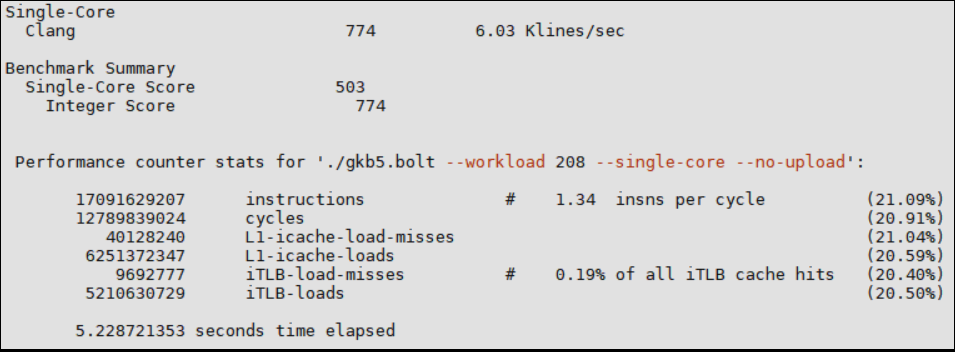
\includegraphics[width=1.0\linewidth]{15}
    }
    \caption{Результаты исполнения оптимизированного Clang теста}\label{fig:ClangRes2}
\end{figure}

Регрессии возникают из-за стандартной проблемы оптимизации на основе профильной информации. Когда исполнение приложения отклоняется от использованного для оптимизации, начинается использование не оптимизированного кода. В случае с BOLT происходит уход исполнения в холодную секцию кода, и средняя температура L1I понижается, приводя к понижению производительности. 

Для решения данной проблемы был реализован режим обработки нескольких трасс одновременно, что исключило регрессии на остальных тестах, а в некоторых случаях и увеличило производительность. Данный режим является аналогом приложения для объединения нескольких профилей, предоставляемого вместе с BOLT.


\section{Вывод по главе}\label{sec:ch3/sect5}
В третьей главе были исследованы существующие проблемы бинарного оптимизатора BOLT, не позволяющие полноценно оптимизировать приложения под ARM архитектуру. В результате проделанной работы удалось реализовать альтернативный способ сбора информации с использованием динамической бинарной инструментации. Исправлены возникающие для данной архитектуры проблемы, связанные с особенностью кодировки команд. Добавлена верификация оптимизированного бинарного файла. Подход протестирован на синтетических тестах и наборе тестов производительности GeekBench и показал ожидаемые результаты.

\clearpage
